% Original Author: GitHub @leowrs (https://github.com/leowrs)
\documentclass[UTF8,a4paper,12pt]{ctexart}

\usepackage{geometry}
\usepackage{setspace}
\usepackage{graphicx}
\usepackage{booktabs}
\usepackage{tabularx}
\usepackage{array}
\usepackage{xcolor}
\usepackage{caption}
\usepackage{enumitem}
\usepackage{fancyhdr}
\usepackage{hyperref}
\usepackage{url}

\geometry{top=2.6cm,bottom=2.6cm,left=3.0cm,right=3.0cm}
\setCJKmainfont[BoldFont=SimHei]{SimSun}
\setCJKsansfont{SimHei}
\setmainfont{Times New Roman}
\newCJKfontfamily\coverfont{STLiti}
\linespread{1.35}
\setlength{\parindent}{2em}
\setlength{\parskip}{0.25em}
\setlength{\headheight}{15pt}
\renewcommand{\arraystretch}{1.25}

\definecolor{seublue}{HTML}{1F4D78}
\definecolor{lightblue}{HTML}{F4F6F9}
\hypersetup{
  colorlinks=true,
  linkcolor=seublue,
  urlcolor=seublue,
  citecolor=seublue,
  pdfauthor={课程报告},
  pdftitle={从视觉基础模型到世界模型：2023—2026年计算机视觉算法与技术最新进展综述}
}
\captionsetup{font=small,labelfont=bf}
\setlist[itemize]{leftmargin=2em,itemsep=0.15em,topsep=0.2em}

\pagestyle{fancy}
\fancyhf{}
\fancyhead[C]{\small 从视觉基础模型到世界模型：计算机视觉算法与技术最新进展综述}
\fancyfoot[C]{\small \thepage}
\renewcommand{\headrulewidth}{0.4pt}

\newcolumntype{Y}{>{\raggedright\arraybackslash}X}
\newcolumntype{C}[1]{>{\centering\arraybackslash}p{#1}}
\newcommand{\model}[1]{\textsf{#1}}

\begin{document}

\begin{titlepage}
  \thispagestyle{empty}
  \begin{center}
    
\includegraphics[width=14.5cm]{seu_cover_header.png}
    \vspace{0.35cm}

    {\coverfont\zihao{1} 计算机视觉基础\par}
    \vspace{0.55cm}
    {\coverfont\zihao{1} 课程实验报告\par}
    \vspace{1.5cm}
    {\heiti\zihao{3} 从视觉基础模型到世界模型：\par}
    \vspace{0.25cm}
    {\heiti\zihao{3} 2023—2026年计算机视觉算法与技术最新进展综述\par}
  \end{center}
  \vspace{1.4cm}
  \begin{center}
  \begin{tabular}{C{3.2cm}p{9.2cm}}
    \toprule
    \textbf{题目} & 介绍算法与技术的最新进展 \\
    \midrule
    \textbf{专业} & 英语+信息工程专业 \\
    \textbf{组员} & — @leowrs \\
     & — 组员A \\
    \textbf{任课教师} & 陆建 \\
    \bottomrule
  \end{tabular}
  \end{center}
  \vfill
  \begin{center}
    {\large 主题选择：介绍算法与技术的最新进展（含思政内容）}
  \end{center}
\end{titlepage}

\pagenumbering{Roman}
\section*{摘要}
2023年以来，计算机视觉的主线已经从单一任务模型转向视觉基础模型、视觉语言模型、生成式视频模型、三维几何模型和具身智能模型的融合演进。以\model{DINOv2}、\model{SAM 2}、\model{Florence-2}为代表的视觉基础模型，通过大规模自监督学习、提示式交互和统一任务表示，使检测、分割、描述和跟踪不再完全依赖“一个任务训练一个模型”的范式。以\model{Qwen2.5-VL}、\model{Gemini 1.5}、\model{GPT-4o}和\model{LLaVA-OneVision}为代表的视觉语言模型，把图像、文档、视频、音频和文本纳入统一推理框架，动态分辨率、超长上下文和多模态指令遵循成为新的能力核心。与此同时，\model{Stable Diffusion 3}、\model{Sora}、\model{Movie Gen}等模型推动视觉生成从静态图像走向长视频、音画同步和可编辑媒体；\model{3D Gaussian Splatting}、\model{pixelSplat}、\model{VGGT}等技术则把实时三维重建、多视图几何和可交互场景表示推向应用前沿。更进一步，\model{OpenVLA}、$\pi_0$和\model{V-JEPA 2}显示出视觉模型正在从“看懂”走向“预测、规划和行动”。本文围绕上述技术路线，分析最新算法机制、代表模型、应用价值与风险挑战，并结合人工智能治理、科技自立自强和智能向善等要求，讨论计算机视觉发展应坚持的价值导向。

\noindent\textbf{关键词（关键字）：}计算机视觉；视觉基础模型；视觉语言模型；生成式视频；三维重建；具身智能；人工智能治理

\newpage
\tableofcontents
\newpage

\section*{小组分工}
\addcontentsline{toc}{section}{小组分工}
\begin{table}[h]
\centering
\begin{tabularx}{\textwidth}{C{3.5cm}Y}
\toprule
\textbf{成员} & \textbf{主要分工} \\
\midrule
— @leowrs & 承担50\%工作量：资料检索、论文阅读、视觉基础模型与视觉语言模型部分整理、正文撰写与终稿校对。 \\
— 组员A & 承担50\%工作量：生成式视觉、三维视觉与具身智能部分整理、图表制作、参考文献核对与格式检查。 \\
\bottomrule
\end{tabularx}
\end{table}

\newpage
\pagenumbering{arabic}

\section{引言}
传统计算机视觉课程通常从图像滤波、边缘检测、特征匹配、相机标定和图像配准讲起。这些内容构成了视觉系统的几何与信号处理基础：图像如何被采样，像素如何被增强，多个视角如何对齐，三维信息如何从二维投影中恢复。但近三年的研究表明，视觉技术的前沿已经发生明显转向：模型不再只学习某个封闭任务的判别边界，而是通过海量图像、视频、文本和交互数据学习通用表征，并用提示、语言或动作把能力迁移到新任务中。

因此，讨论“算法与技术的最新进展”不能只列举若干模型排行榜。更重要的问题是：这些模型为什么能统一多种视觉任务？视觉语言模型如何突破固定分辨率和短上下文限制？生成式视频为什么被称为世界模拟器？三维重建和具身智能又如何把视觉从识别系统推进到行动系统？本文以截至2026年6月可公开核验的论文和官方技术报告为依据，按“表征—理解—生成—三维—行动”的顺序梳理最新进展。

\section{计算机视觉算法演进的总体趋势}
第一条趋势是基础模型化。\model{DINOv2}通过大规模自监督学习获得稳健视觉特征，证明在没有人工标注类别的情况下，视觉编码器仍能迁移到分类、检索、密集预测等任务\cite{dinov2}。\model{SAM 2}进一步把“可提示分割”从静态图像扩展到视频，利用流式记忆机制在视频中保持目标身份和交互效率\cite{sam2}。\model{Florence-2}则把检测、描述、定位、分割等任务统一为提示到序列的框架，并通过大规模自动标注数据训练统一视觉表示\cite{florence2}。这些工作共同说明，视觉模型正在从专用工具变成可组合的通用能力层。

第二条趋势是多模态推理化。视觉语言模型不再只是给图片配字幕，而是要理解图表、文档、视频事件、屏幕界面和现实场景。\model{Qwen2.5-VL}在动态分辨率、细粒度定位、文档理解和长视频理解方面继续增强\cite{qwen25vl}；\model{Gemini 1.5}把百万级上下文引入多模态场景\cite{gemini15}；\model{GPT-4o}强调原生多模态交互与实时响应\cite{gpt4o}。这意味着视觉系统的输出从“类别标签”变成了“可解释、可追问、可执行的语义信息”。

第三条趋势是生成与几何融合。\model{Stable Diffusion 3}采用多模态扩散Transformer和整流流机制，提高了高分辨率图像生成的可扩展性\cite{sd3}；\model{Sora}和\model{Movie Gen}把视频压缩为时空潜变量再进行生成，使视频模型开始具备镜头连贯性、物体持久性和可编辑能力\cite{sora,moviegen}。与此同时，\model{3D Gaussian Splatting}实现实时新视角渲染\cite{gs3d}，\model{VGGT}尝试用统一Transformer处理相机位姿、深度和点云等几何任务\cite{vggt}。视觉算法正在同时追求语义理解、物理一致性和三维可交互表示。

\begin{figure}[htbp]
  \centering
  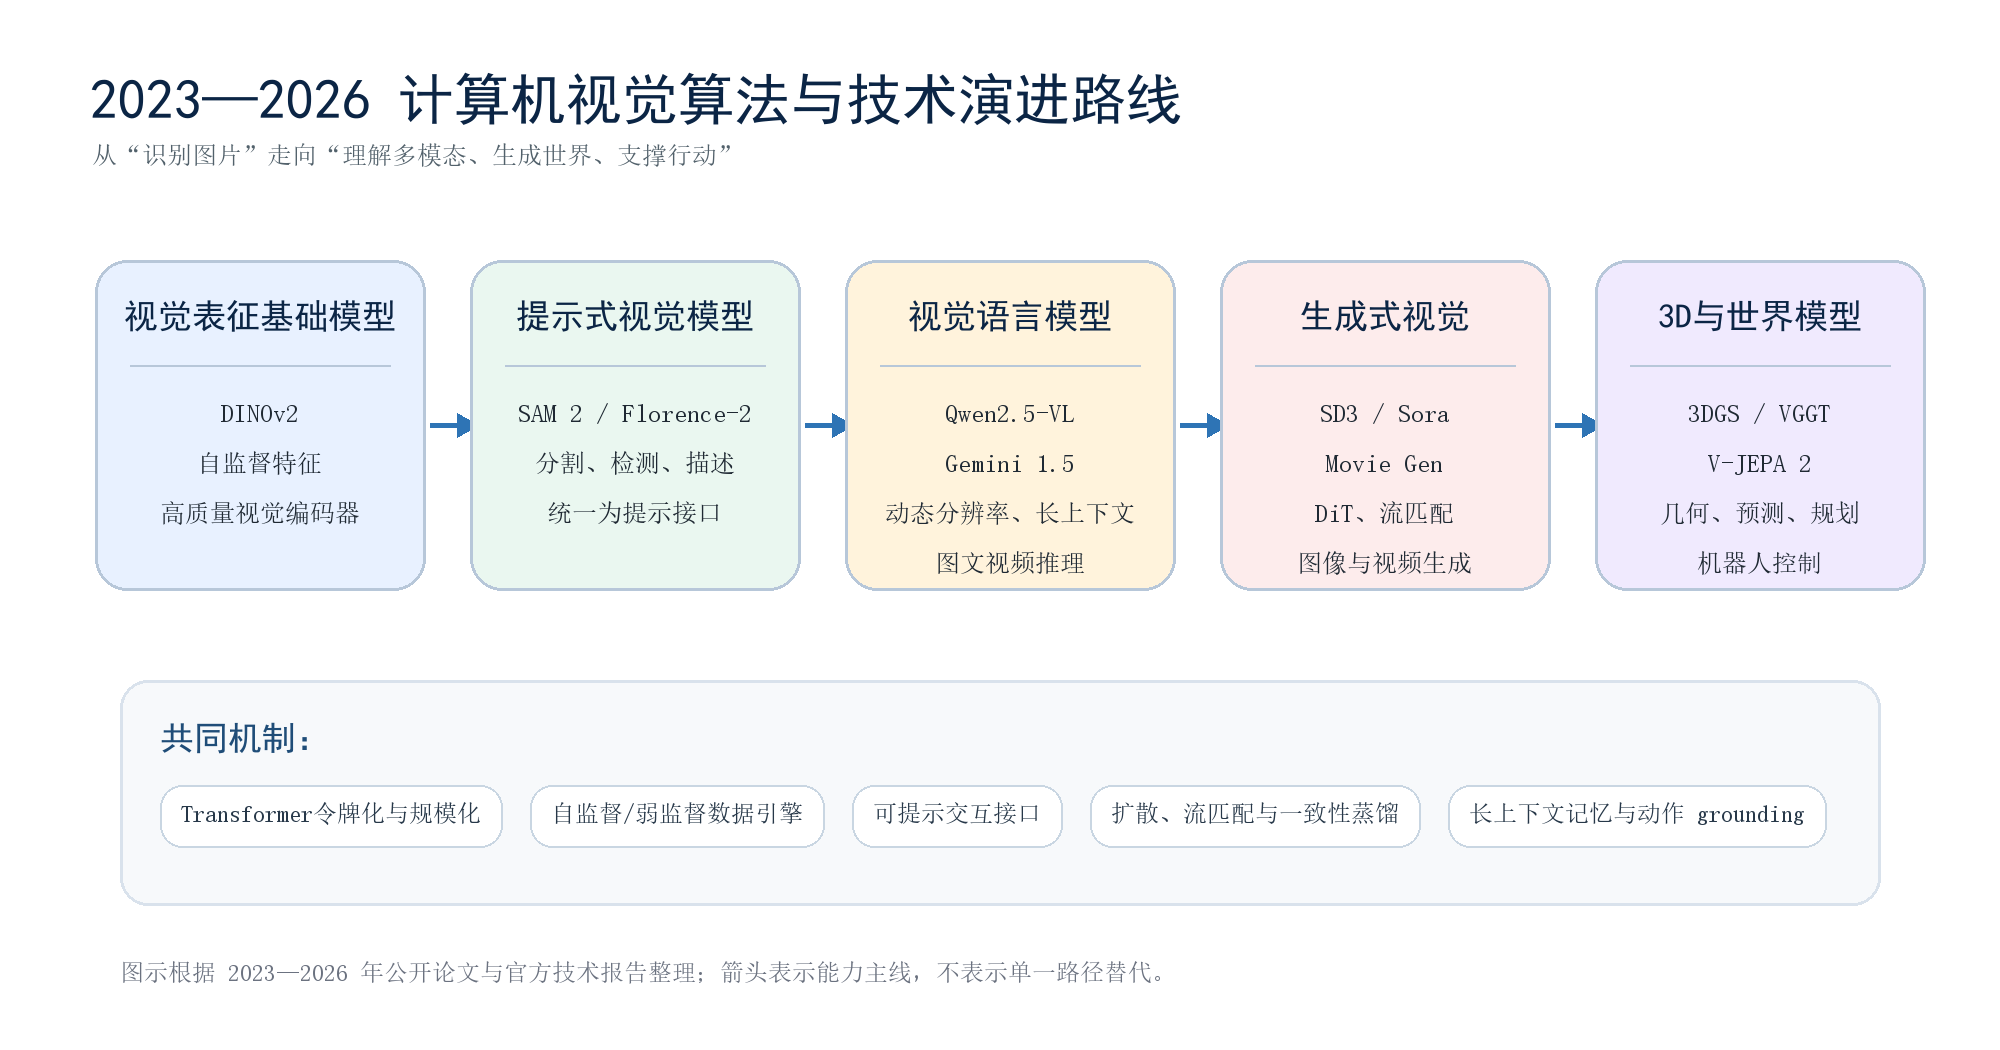
\includegraphics[width=\textwidth]{cv_foundation_model_roadmap.png}
  \caption{2023—2026年计算机视觉算法与技术演进路线}
  \label{fig:roadmap}
\end{figure}

\begin{table}[htbp]
\centering
\small
\caption{计算机视觉最新进展的主线归纳}
\begin{tabularx}{\textwidth}{C{2.2cm}Y Y Y}
\toprule
\textbf{技术主线} & \textbf{代表模型/技术} & \textbf{核心机制} & \textbf{意义} \\
\midrule
通用表征 & \model{DINOv2}、\model{SAM 2}、\model{Florence-2} & 自监督学习、提示式分割、统一任务序列化 & 降低迁移成本，使视觉能力可复用 \\
多模态推理 & \model{Qwen2.5-VL}、\model{Gemini 1.5}、\model{GPT-4o}、\model{LLaVA-OneVision} & 动态分辨率、长上下文、图文视频联合推理 & 视觉系统从识别走向解释、对话和任务执行 \\
开放词汇与密集预测 & \model{YOLO-World}、\model{Depth Anything V2} & 文本条件检测、大规模弱监督/合成数据 & 减少类别封闭假设，提升真实场景适应性 \\
生成式视觉 & \model{SD3}、\model{PIXART-$\delta$}、\model{DyDiT}、\model{Sora}、\model{Movie Gen} & DiT、整流流、一致性蒸馏、时空潜变量 & 提高内容生产、仿真和视频编辑能力 \\
三维与具身智能 & \model{3DGS}、\model{pixelSplat}、\model{VGGT}、\model{OpenVLA}、$\pi_0$、\model{V-JEPA 2} & 显式高斯表示、多视图Transformer、VLA动作头、预测式世界模型 & 连接机器人、AR/VR和物理世界任务 \\
\bottomrule
\end{tabularx}
\end{table}

\section{正文：算法与技术的最新进展}
\subsection{视觉基础模型：从专用网络到通用表征}
早期深度视觉模型通常围绕ImageNet分类、COCO检测或特定分割数据集优化，模型结构与训练目标高度绑定。\model{DINOv2}的意义在于，它把自监督视觉特征训练提升到基础模型层面：模型不依赖人工类别标签，而是通过视觉自身的相似性、局部—全局一致性和大规模数据过滤形成可迁移特征\cite{dinov2}。这种特征对下游任务有两个价值：一是减少标注成本，二是让不同任务共享同一个视觉编码器，便于工业系统中的统一部署。

\model{SAM 2}代表了另一个方向：不是只输出一个固定类别，而是让用户用点、框、掩码或历史记忆提示模型分割目标。相比图像版SAM，\model{SAM 2}面向视频引入streaming memory，使模型能在连续帧中保持目标信息，并通过model-in-the-loop数据引擎不断改善交互质量\cite{sam2}。这类模型适合医疗影像轮廓标注、工业缺陷定位、视频编辑和遥感对象提取等场景。它的启示是，未来视觉模型的交互方式将更接近“协作式标注助手”，而不只是一次性预测器。

\model{Florence-2}进一步提出统一任务接口：把视觉任务都表示为文本提示和序列输出，例如“请描述图像”“请找出某物体位置”“请输出区域掩码”等\cite{florence2}。这与大语言模型的指令范式相似，使视觉系统能够通过自然语言或结构化提示选择任务。从课程知识角度看，这并没有否定传统图像处理和几何视觉，而是把底层特征、区域、边界和语义包装成更高层的可调用能力。

\subsection{视觉语言模型：从看图问答到多模态推理}
视觉语言模型的发展速度尤其快。2024年的\model{Qwen2-VL}强调“任意分辨率”感知，通过动态分辨率把不同尺寸图像转化为不同数量视觉token，并结合多维旋转位置编码处理二维图像和视频时间信息\cite{qwen2vl}。2025年的\model{Qwen2.5-VL}继续加强文档解析、细粒度定位、视频事件理解和视觉agent能力\cite{qwen25vl}。这类设计解决了一个实际痛点：真实图像并不总是固定尺寸，文档截图、医学图像、监控画面和长视频都可能因为缩放而丢失关键信息。

\model{Gemini 1.5}展示了另一种能力路线：超长上下文。论文报告模型能够处理包含长文本、长视频、音频和代码的百万级上下文\cite{gemini15}。对于计算机视觉而言，长上下文意味着模型可以一次性理解更完整的过程，例如一段实验视频的全部步骤、一场课堂录屏的关键节点，或一组多视角图像之间的关系。\model{GPT-4o}和其他原生多模态模型则强调低延迟音视频交互，使视觉理解更接近实时人机协作\cite{gpt4o}。

开源视觉语言模型也在缩小与闭源模型的差距。\model{LLaVA-OneVision}通过统一单图、多图和视频任务迁移，说明视觉语言模型可以从单图对话扩展到跨媒体理解\cite{llavaov}。\model{PaliGemma 2}和\model{Idefics2}等模型表明，紧凑视觉编码器、语言模型和高质量训练流程结合后，也能在OCR、图像描述、细粒度识别和文档理解中取得实用效果\cite{paligemma2,idefics2}。这对教学和科研尤其重要，因为开放模型便于复现实验、理解机制和构建国产化应用。

\subsection{开放词汇检测、分割与几何估计}
真实世界的视觉任务往往存在开放类别。传统检测器需要预先定义类别集合，遇到训练集中没有的对象就会失效。\model{YOLO-World}把文本嵌入与实时检测框架结合，使检测器能够根据文本提示识别开放词汇目标\cite{yoloworld}。这类方法适合仓储盘点、安防巡检、机器人抓取等场景，因为用户可以临时指定要找的对象，而不是重新标注并训练整个检测器。

密集几何估计也出现基础模型化趋势。\model{Depth Anything V2}通过大规模数据和更强教师模型提升单目深度估计泛化能力\cite{depthanythingv2}。单目深度本质上是不适定问题，因为一张图像缺少真实尺度；但大规模预训练能学习常见场景的几何先验，使模型在自动驾驶、室内导航、AR测量和三维重建中提供更稳定的初值。需要注意的是，深度基础模型仍可能在透明物体、反光表面、极端光照和罕见场景中失效，因此工程应用必须结合相机标定、多传感器融合和异常检测。

\subsection{生成式图像与视频：从合成内容到世界模拟}
生成式视觉的核心变化是骨干结构和采样方式的变化。\model{Stable Diffusion 3}使用多模态扩散Transformer与整流流训练，说明扩散模型正在从U-Net主干走向Transformer主干，并更重视文本—图像对齐和高分辨率生成\cite{sd3}。\model{PIXART-$\delta$}通过潜空间一致性模型把高质量图像生成压缩到少步采样\cite{pixartdelta}，\model{DyDiT}则尝试根据时间步和空间token动态调整扩散Transformer计算量\cite{dydit}。这些工作说明生成模型的竞争不再只是“画得更逼真”，还包括更快、更可控、更低成本。

视频生成是近年最受关注的方向。\model{Sora}官方技术报告将视频和图像表示为时空patch，并在压缩后的潜空间中训练生成模型，使同一框架能够处理不同长度、分辨率和宽高比的视频\cite{sora}。\model{Movie Gen}进一步覆盖文本生成视频、个性化视频、视频编辑和音频生成，被定位为一组媒体基础模型\cite{moviegen}。\model{Veo}系列则展示了高质量视频生成、镜头控制和声音结合能力\cite{veo}。这些模型让视觉生成从静态图片合成走向内容生产流程，但也带来深度伪造、版权归属、训练数据透明度和物理一致性不足等问题。

把视频生成称为“世界模拟器”并不意味着模型真正理解物理定律。更准确地说，模型学到了大量视觉动态的统计规律：物体如何移动，镜头如何变化，动作如何影响场景。当这些规律足够强时，模型可以为机器人训练、自动驾驶仿真和影视预演提供低成本数据。但它仍可能在因果关系、物体守恒、长期一致性和可控性方面出错，所以不能把生成视频直接等同于可靠仿真。

\subsection{三维重建、多视图视觉与可编辑资产}
三维视觉长期依赖多视图几何、SLAM、NeRF和深度传感器。2023年的\model{3D Gaussian Splatting}用显式三维高斯表示场景，在保证较高渲染质量的同时实现实时新视角渲染\cite{gs3d}。与需要大量体渲染采样的NeRF相比，高斯表示更适合交互式浏览、编辑和AR/VR显示。\model{pixelSplat}则从图像对直接预测3D Gaussian，使可泛化三维重建更接近即时生成\cite{pixelsplat}。

2025年的\model{VGGT}把视觉几何任务进一步统一化：模型尝试从一个或多个视图中预测相机参数、深度图、点云和跟踪信息\cite{vggt}。这与课程中相机标定、图像配准和三维重建的知识直接相关。传统方法强调几何约束和优化，基础模型强调数据驱动的先验与端到端预测。更合理的未来方向不是二选一，而是把深度学习的强先验与几何约束结合起来：用模型给出初值和语义理解，用几何优化保证尺度、位姿和一致性。

\subsection{世界模型与具身智能：从理解到行动}
计算机视觉的最终目标之一是让机器理解并参与真实世界。\model{OpenVLA}把视觉语言模型接入机器人动作输出，形成开源视觉—语言—动作模型\cite{openvla}；$\pi_0$使用视觉语言条件和flow matching策略学习通用机器人控制\cite{pi0}。这些方法把视觉输入、语言指令和低层动作连接起来，使模型不只回答“图中有什么”，还要决定“接下来怎么做”。

\model{V-JEPA 2}代表预测式世界模型路线：模型通过自监督视频学习形成对未来状态和场景变化的预测能力，并把理解、预测和规划连接起来\cite{vjepa2}。\model{Genie 2}则把世界模型用于可交互环境生成，强调从图像或文本提示中生成可操作的虚拟世界\cite{genie2}。这说明视觉算法正在进入一个新的问题域：模型需要理解时间、因果、动作结果和任务目标。从算法角度看，这要求更好的长时记忆、物理一致性、可验证规划和跨机器人平台泛化。

\begin{table}[htbp]
\centering
\small
\caption{代表性最新视觉算法与技术对照}
\begin{tabularx}{\textwidth}{C{2.45cm}C{1.75cm}C{2.05cm}Y Y}
\toprule
\textbf{模型/技术} & \textbf{年份} & \textbf{类型} & \textbf{核心机制} & \textbf{典型应用} \\
\midrule
\model{DINOv2} & 2023 & 自监督视觉表征 & 无标注特征学习、数据过滤、大规模ViT & 迁移分类、检索、密集预测 \\
\model{SAM 2} & 2024 & 提示式图像/视频分割 & 流式记忆、交互提示、数据引擎 & 视频目标分割、医学/工业标注 \\
\model{Qwen2.5-VL} & 2025 & 视觉语言模型 & 动态分辨率、定位、长视频和文档理解 & 多模态助手、OCR、视觉agent \\
\model{Sora}/\model{Movie Gen} & 2024 & 视频生成 & 时空潜变量、DiT/扩散、音视频生成与编辑 & 内容创作、仿真、视频后期 \\
\model{3DGS}/\model{VGGT} & 2023/2025 & 三维视觉 & 显式高斯表示、多视图几何Transformer & AR/VR、数字孪生、机器人感知 \\
\model{OpenVLA}/$\pi_0$ & 2024 & 具身智能 & VLM接动作头、flow policy、机器人演示数据 & 机器人控制、通用操作任务 \\
\bottomrule
\end{tabularx}
\end{table}

\section{从课程基础到前沿模型的知识连接}
本课程前半部分讲到的图像处理基础、相机模型、相机标定和图像配准，并不是被大模型时代淘汰的旧知识。相反，越是复杂的视觉基础模型，越需要这些基础概念来解释其输入、约束和失效边界。许多新模型在论文中看起来是端到端系统，但工程落地时仍要回答三个传统问题：图像信号是否可靠，视角和尺度是否可解释，多帧或多视图之间是否一致。没有这些基础，模型输出就容易停留在“看起来合理”，而不能成为可验证、可部署的视觉系统。

首先，图像处理基础仍然决定模型输入质量。传统课程中的去噪、增强、直方图均衡、边缘和纹理分析，本质上是在改善像素分布和局部结构，使后续算法更容易提取稳定特征。深度视觉模型虽然把滤波器、边缘和纹理特征交给网络自动学习，但它们仍然受到噪声、模糊、曝光不足、运动拖影和压缩伪影影响。例如工业相机拍摄高速流水线时，若光照不稳定或快门设置不当，\model{SAM 2}的分割边界、\model{YOLO-World}的检测框和视觉语言模型的文本解释都可能同时退化。因此，现代视觉系统并不是“直接把图片丢给大模型”，而是需要在采集、预处理、模型推理和后处理之间建立完整链路。

其次，相机模型和相机标定仍是三维视觉的坐标基础。课程中的针孔相机模型、内参、外参、畸变校正和重投影误差，回答的是二维图像如何对应三维空间的问题。\model{VGGT}、\model{Depth Anything V2}、\model{3D Gaussian Splatting}等前沿模型能够从数据中学习几何先验，但如果要进行真实尺度测量、机器人抓取或AR叠加，仍必须知道相机坐标系与世界坐标系之间的关系。单目深度模型可以给出相对深度趋势，却未必给出可直接用于机械臂控制的米制尺度；高斯重建可以生成逼真视角，却可能在尺度漂移或相机位姿不准时产生局部扭曲。由此可见，几何视觉的价值从“手工设计完整算法”转向“为学习模型提供约束和校验”。

再次，图像配准和特征匹配是视频理解、三维重建和世界模型的隐含基础。传统配准关注关键点、描述子、单应矩阵、基础矩阵和光流估计，目标是让不同图像或不同帧中的同一结构对齐。视频基础模型虽然使用Transformer token、时序位置编码或记忆模块，但它们仍要解决同一个问题：跨帧目标如何保持身份，遮挡后如何恢复，摄像机运动和物体运动如何区分。\model{SAM 2}的streaming memory可以看作一种学习到的跨帧配准和目标记忆；视频生成模型中的时空patch建模，也是在高维潜空间中维持帧间一致性。若模型无法保持配准一致，生成视频就会出现物体形变、纹理跳变或身份漂移。

最后，误差分析和鲁棒性评估是传统视觉与基础模型共同面对的问题。相机标定中有重投影误差，图像配准中有匹配误差，深度估计中有尺度误差，视觉语言模型中则有语义幻觉和定位错误。不同任务的误差形式不同，但都需要被量化和追踪。一个可靠系统不应只输出答案，还应输出置信度、失败提示和可复核证据。例如在医疗图像分割中，模型给出病灶区域后应保留原图、提示点、版本号和人工修订记录；在自动驾驶仿真中，世界模型生成的视频不能只看视觉质量，还要评估交通规则、物体轨迹和碰撞逻辑是否一致。

\begin{table}[htbp]
\centering
\small
\caption{课程基础知识与最新视觉模型的对应关系}
\begin{tabularx}{\textwidth}{C{2.5cm}Y Y Y}
\toprule
\textbf{课程知识点} & \textbf{核心问题} & \textbf{前沿模型中的体现} & \textbf{工程启示} \\
\midrule
图像处理基础 & 如何获得清晰、稳定、可分析的像素输入 & 视觉编码器对噪声、模糊和曝光变化仍敏感 & 采集与预处理质量会直接影响模型上限 \\
相机模型与标定 & 二维图像如何对应三维空间坐标 & \model{VGGT}、\model{Depth Anything V2}需要几何尺度校验 & 学习模型适合给初值，真实测量仍要几何约束 \\
图像配准 & 多视角、多帧之间如何保持对应关系 & \model{SAM 2}记忆模块和视频模型时空token都需保持一致性 & 视频理解和生成要同时关注语义与时序稳定 \\
三维重建 & 如何从图像恢复可交互空间表示 & \model{3DGS}、\model{pixelSplat}把场景表示推向实时渲染 & 显式三维表示更利于编辑、导航和机器人应用 \\
误差分析 & 预测结果是否可信、何时失效 & VLM幻觉、深度尺度漂移、生成视频物理错误 & 必须建立置信度、人工复核和持续监测机制 \\
\bottomrule
\end{tabularx}
\end{table}

\section{应用价值与现实挑战}
从应用角度看，最新视觉算法的价值主要体现在四类场景。第一是工业制造。开放词汇检测、视频分割和三维重建可以用于缺陷检测、工件定位、产线安全和数字孪生。第二是医疗与公共服务。提示式分割和多模态文档理解可辅助医生标注病灶、整理影像报告，但必须由专业人员复核，不能替代诊断责任。第三是交通与城市治理。深度估计、视频理解和世界模型可服务自动驾驶仿真、道路风险识别和应急响应。第四是教育、文化和科研。生成式视觉和三维重建可以用于虚拟实验、文物数字化、课程可视化和科研数据增强。

在智能制造场景中，视觉基础模型可以改变传统质检流程。过去一条产线往往需要为每类缺陷分别采集样本、标注数据、训练检测器，遇到新产品或新缺陷时还要重新开发。开放词汇检测和提示式分割使系统能够先用文本或少量交互指定目标，再由模型给出候选区域，最后结合规则、测量和人工复核完成判定。若进一步加入三维重建，系统还能判断零件姿态、装配间隙和表面形变。这样的流程更适合小批量、多品种生产，但它对相机标定、光照稳定、缺陷样本管理和误报控制提出了更高要求。

在医疗与公共服务场景中，计算机视觉的价值不在于替代医生，而在于提高信息处理效率。以医学影像为例，\model{SAM 2}一类模型可以辅助轮廓勾画，视觉语言模型可以帮助整理影像描述和检查记录，三维重建可以辅助术前规划。但医学场景高度敏感，模型必须满足可追溯、可复核和隐私保护要求。尤其是视觉语言模型生成文本时，若把不确定区域描述成确定病灶，或者遗漏关键异常，就会带来严重风险。因此，医疗视觉系统更适合作为“第二读片者”或“标注加速器”，而不是独立决策者。

在交通和城市治理场景中，长视频理解、深度估计和世界模型具有现实意义。城市摄像头、车载摄像头和无人机视频通常包含长时间、多目标、多视角信息，仅靠单帧检测难以判断风险演化。视觉语言模型可以把长视频转化为事件描述，深度模型可以估计道路空间结构，世界模型可以生成罕见危险场景用于仿真训练。但交通系统必须强调实时性和安全冗余：模型推理延迟、夜间雨雾天气、遮挡和镜头污染都可能影响结果。真正可用的系统通常需要视觉模型、雷达、地图、规则引擎和人工调度协同工作。

在教育、文化和科研场景中，生成式视觉与三维视觉能够降低知识可视化门槛。教师可以用生成式图像和视频解释抽象概念，用三维重建展示文物、建筑或实验装置；科研人员可以用合成数据补充罕见样本，用视频模型进行实验方案预演。但这些应用同样需要边界：生成内容必须标注来源，不能把生成图像当作真实实验结果；文化遗产数字化要尊重版权和文物保护规范；教育材料要避免把模型生成的错误细节包装成权威知识。

\begin{table}[htbp]
\centering
\small
\caption{典型应用场景、可用技术与落地约束}
\begin{tabularx}{\textwidth}{C{2.3cm}Y Y Y}
\toprule
\textbf{场景} & \textbf{可用技术} & \textbf{主要收益} & \textbf{关键约束} \\
\midrule
智能制造 & 开放词汇检测、提示式分割、三维重建 & 缩短新缺陷适配周期，提升质检自动化 & 光照、标定、误报率、产线实时性 \\
医疗影像 & 视频/图像分割、VLM报告辅助、三维可视化 & 加速标注和报告整理，辅助术前分析 & 隐私保护、医生复核、责任归属 \\
交通治理 & 长视频理解、深度估计、世界模型仿真 & 识别风险事件，生成罕见场景数据 & 低延迟、多传感器冗余、极端天气鲁棒性 \\
教育科研 & 生成式图像视频、3DGS、可交互可视化 & 降低可视化和实验演示成本 & 内容真实性标注、版权和学术诚信 \\
文化遗产 & 多视图重建、三维资产生成、图像修复 & 支持数字保护、展示和远程传播 & 采集规范、历史真实性、数据长期保存 \\
\bottomrule
\end{tabularx}
\end{table}

挑战同样突出。首先是数据与隐私问题。视觉模型训练常依赖海量图像和视频，若数据来源、授权和脱敏流程不清晰，容易侵犯个人信息和知识产权。其次是可靠性问题。视觉语言模型可能产生幻觉，生成式视频可能违反物理规律，深度估计和三维重建可能在特殊材质或极端场景中失败。再次是算力与能耗问题。基础模型规模越大，对训练算力、推理成本和部署设备的要求越高。最后是评价体系问题。很多榜单只衡量静态数据集表现，却难以评估模型在真实开放环境中的安全性、稳定性和可解释性。

因此，未来视觉系统的工程落地应采用“模型能力 + 任务约束 + 人工复核 + 持续评估”的方式。例如在工业质检中，模型可先给出缺陷候选区域，再由规则或人工复核关键样本；在医疗场景中，模型输出应作为辅助信息并保留审计记录；在生成式内容场景中，应加入水印、来源标注和滥用检测。这样的系统设计比单纯追求模型排行榜更符合现实需求。

\section{评价方法与实验验证思路}
课程报告如果只介绍模型能力，容易忽略一个关键问题：如何判断这些能力是否可靠。传统计算机视觉常用准确率、召回率、IoU、平均精度、重投影误差等指标评价单一任务；基础模型和多模态模型则需要更综合的评价体系。原因在于，这些模型往往同时处理图像、文本、视频和动作，输出也可能是掩码、框、描述、代码或控制指令。单一指标无法覆盖其真实行为。

第一类评价是任务性能评价。对于检测和分割，仍可使用mAP、IoU、Dice等指标；对于深度估计，可使用绝对相对误差、尺度一致性和边缘保持能力；对于视觉语言模型，可评估图像问答、OCR、定位、图表理解和长视频事件识别。任务性能评价的优点是可量化、可对比，缺点是容易受数据集分布影响。模型在公开榜单上表现好，并不代表它在学校实验室、工厂车间或医院设备中同样可靠。

第二类评价是鲁棒性评价。真实环境中的图像会遇到噪声、低照度、遮挡、压缩、运动模糊和域偏移。对于视觉基础模型，应该测试不同相机、不同光照、不同分辨率下的稳定性；对于生成式视频模型，应该测试长时间一致性、物体守恒和动作因果关系；对于VLA机器人模型，应该测试指令变化、物体位置变化和异常中断时的恢复能力。鲁棒性评价往往比平均精度更能反映系统是否能落地。

第三类评价是安全与责任评价。视觉语言模型可能编造不存在的物体，生成式模型可能生成误导内容，监控视觉系统可能造成隐私泄露。安全评价需要检查模型是否能拒绝不合规请求，是否会泄露训练数据中的个人信息，是否能给出不确定性提示，是否保留人工复核入口。对于涉及公共安全、医疗和未成年人的应用，安全评价应高于普通性能评价。

第四类评价是成本评价。基础模型通常需要较高算力，但很多视觉任务运行在边缘设备、移动终端或机器人上。一个模型即使精度高，如果推理延迟过长、显存占用过大、能耗过高，也可能无法部署。因此，课程报告中的“先进”不应只理解为规模最大或效果最好，还应包括在给定资源下的性价比。动态扩散Transformer、一致性蒸馏、小型VLM和模型量化等方向，正是为了解决这一矛盾。

\begin{table}[htbp]
\centering
\small
\caption{视觉基础模型的多维评价框架}
\begin{tabularx}{\textwidth}{C{2.5cm}Y Y}
\toprule
\textbf{评价维度} & \textbf{关注问题} & \textbf{可采用的方法} \\
\midrule
任务性能 & 模型在标准任务上是否有效 & mAP、IoU、OCR准确率、VQA正确率、深度误差等 \\
鲁棒性 & 环境变化后是否稳定 & 噪声、模糊、遮挡、低照度、跨设备和跨场景测试 \\
一致性 & 多帧、多视角和生成内容是否前后一致 & 视频目标保持、三维重投影、长视频事件链检查 \\
安全治理 & 是否存在幻觉、隐私和滥用风险 & 拒答测试、水印检测、审计记录、人工复核流程 \\
部署成本 & 是否能在实际设备中运行 & 延迟、显存、能耗、吞吐量和边缘端适配测试 \\
\bottomrule
\end{tabularx}
\end{table}

若要把本文扩展成后续实验或演示，可以选择一个小而完整的验证任务。例如，用公开图片测试\model{SAM 2}或类似分割模型的提示交互，用不同光照和噪声版本比较分割稳定性；或者选取一组多视角图片，用三维重建工具生成可浏览场景，再分析相机位姿和重建质量；还可以选择一段课堂或交通短视频，让视觉语言模型总结事件并人工核对错误。这样的实验不一定追求大规模训练，但能体现课程中“输入—模型—输出—评价”的完整闭环。

\section{思政融入：价值导向、责任边界与科技自立自强}
计算机视觉的最新进展不仅是算法问题，也关系到国家科技竞争力、数字经济发展和社会治理。《新一代人工智能发展规划》提出要把人工智能作为推动科技跨越发展、产业优化升级和生产力整体跃升的重要战略技术\cite{aiplan}。视觉基础模型、三维重建和具身智能正是人工智能从互联网应用走向实体经济的重要接口：它们让机器能够感知生产线、交通道路、农田矿山和医疗影像。学习这些技术，不应停留在调用模型接口，而应理解数据、算法、算力和应用场景之间的系统关系，增强科技自立自强意识。

同时，技术越强，责任边界越重要。生成式视觉能够降低创作门槛，也可能被用于深度伪造、谣言传播和侵犯肖像权；视觉监控能够提升公共安全，也可能造成过度采集和算法歧视；视觉语言模型能提升服务效率，也可能在关键场景中给出不可靠建议。《生成式人工智能服务管理暂行办法》强调生成式人工智能服务应遵守法律法规、尊重社会公德伦理、保护个人信息和知识产权\cite{genai2023}。这提示我们，算法研究必须与数据治理、安全评估、可解释性和责任追溯同步推进。

从青年学生角度看，思政要求不是在技术报告末尾附加口号，而是贯穿问题选择、方法设计和应用落地。在选择研究方向时，应关注服务国家重大需求和人民生活质量的视觉任务，例如智能制造、智慧医疗、灾害监测、无障碍辅助和文化遗产保护。在设计系统时，应坚持以人为本，把人的安全、尊严、隐私和知情权放在效率之前。在评价成果时，应同时看精度、鲁棒性、公平性、能耗和社会影响。只有这样，计算机视觉的最新进展才能真正转化为可信、可控、可持续的生产力。

\section{展望}
第一，视觉模型会继续向统一多模态模型演进。未来模型可能同时处理图像、视频、音频、三维场景、传感器数据和机器人动作，并通过统一接口完成观察、理解、生成和控制。第二，长视频和长期记忆会成为关键能力。真实任务往往持续数分钟甚至数小时，模型需要记住目标、环境变化和任务进度，而不是只理解单帧图像。第三，三维和物理一致性会重新获得重要地位。生成式模型若要服务自动驾驶、机器人和工业仿真，就必须接受几何约束、动力学约束和可验证评估。

第四，高效部署会成为基础研究的重要指标。边缘设备、移动终端和机器人无法承受无限算力，动态计算、模型蒸馏、量化和小模型迁移将持续发展。第五，可信治理会从外部约束变成模型设计的一部分。未来视觉系统需要内置水印、数据来源记录、不确定性估计、拒答机制和审计接口。第六，开源生态和国产模型会更加重要。只有在可复现、可审计、可本地化部署的生态中，视觉算法才能更好服务教育、科研和产业升级。

\section{报告总结}
本文围绕“介绍算法与技术的最新进展”这一主题，梳理了2023—2026年计算机视觉从基础表征到世界模型的主要变化。总体来看，最新进展可以概括为三句话：第一，视觉模型正在基础模型化，分割、检测、描述和几何估计逐渐统一到可提示、可迁移的框架中；第二，视觉语言模型和生成式视频模型正在把视觉系统从静态识别推向多模态推理、内容生成和世界模拟；第三，三维视觉和具身智能正在把视觉能力连接到物理行动，使“看见”最终服务“理解、预测和执行”。

这些进展令人振奋，但也提醒我们不能把算法能力等同于社会价值。优秀的计算机视觉系统既要有高精度和高效率，也要有安全边界、数据合规、可解释机制和面向真实需求的应用设计。对学生而言，学习最新算法的意义不仅是掌握模型名称和论文结论，更是理解技术演进背后的科学问题、工程约束和价值责任。只有把专业学习、国家需求和社会责任结合起来，才能让计算机视觉技术在未来真正发挥积极作用。

\newpage
\begin{thebibliography}{99}
\addcontentsline{toc}{section}{参考文献}
\bibitem{dinov2} Oquab M, Darcet T, Moutakanni T, et al. DINOv2: Learning Robust Visual Features without Supervision[EB/OL]. arXiv:2304.07193, 2023. \url{https://arxiv.org/abs/2304.07193}
\bibitem{sam2} Ravi N, Gabeur V, Hu Y T, et al. SAM 2: Segment Anything in Images and Videos[EB/OL]. arXiv:2408.00714, 2024. \url{https://arxiv.org/abs/2408.00714}
\bibitem{florence2} Xiao B, Wu H, Xu W, et al. Florence-2: Advancing a Unified Representation for a Variety of Vision Tasks[EB/OL]. arXiv:2311.06242, 2023. \url{https://arxiv.org/abs/2311.06242}
\bibitem{yoloworld} Cheng T, Song L, Ge Y, et al. YOLO-World: Real-Time Open-Vocabulary Object Detection[EB/OL]. arXiv:2401.17270, 2024. \url{https://arxiv.org/abs/2401.17270}
\bibitem{qwen2vl} Wang P, Bai S, Tan S, et al. Qwen2-VL: Enhancing Vision-Language Model's Perception of the World at Any Resolution[EB/OL]. arXiv:2409.12191, 2024. \url{https://arxiv.org/abs/2409.12191}
\bibitem{qwen25vl} Bai S, Chen K, Liu X, et al. Qwen2.5-VL Technical Report[EB/OL]. arXiv:2502.13923, 2025. \url{https://arxiv.org/abs/2502.13923}
\bibitem{gemini15} Gemini Team, Georgiev P, Lei V I, et al. Gemini 1.5: Unlocking Multimodal Understanding across Millions of Tokens of Context[EB/OL]. arXiv:2403.05530, 2024. \url{https://arxiv.org/abs/2403.05530}
\bibitem{gpt4o} OpenAI. GPT-4o System Card[EB/OL]. 2024. \url{https://openai.com/index/gpt-4o-system-card/}
\bibitem{llavaov} Li B, Zhang Y, Guo D, et al. LLaVA-OneVision: Easy Visual Task Transfer[EB/OL]. arXiv:2408.03326, 2024. \url{https://arxiv.org/abs/2408.03326}
\bibitem{depthanythingv2} Yang L, Kang B, Huang Z, et al. Depth Anything V2[EB/OL]. arXiv:2406.09414, 2024. \url{https://arxiv.org/abs/2406.09414}
\bibitem{vggt} Wang J, Chen M, Karaev N, et al. VGGT: Visual Geometry Grounded Transformer[EB/OL]. arXiv:2503.11651, 2025. \url{https://arxiv.org/abs/2503.11651}
\bibitem{gs3d} Kerbl B, Kopanas G, Leimkühler T, et al. 3D Gaussian Splatting for Real-Time Radiance Field Rendering[EB/OL]. arXiv:2308.04079, 2023. \url{https://arxiv.org/abs/2308.04079}
\bibitem{pixelsplat} Charatan D, Li S, Tagliasacchi A, et al. pixelSplat: 3D Gaussian Splats from Image Pairs for Scalable Generalizable 3D Reconstruction[EB/OL]. arXiv:2312.12337, 2023. \url{https://arxiv.org/abs/2312.12337}
\bibitem{sd3} Esser P, Kulal S, Blattmann A, et al. Scaling Rectified Flow Transformers for High-Resolution Image Synthesis[EB/OL]. arXiv:2403.03206, 2024. \url{https://arxiv.org/abs/2403.03206}
\bibitem{pixartdelta} Chen J, Wu Y, Luo S, et al. PIXART-$\delta$: Fast and Controllable Image Generation with Latent Consistency Models[EB/OL]. arXiv:2401.05252, 2024. \url{https://arxiv.org/abs/2401.05252}
\bibitem{dydit} Zhao W, Han Y, Tang J, et al. Dynamic Diffusion Transformer[EB/OL]. arXiv:2410.03456, 2024. \url{https://arxiv.org/abs/2410.03456}
\bibitem{sora} OpenAI. Video Generation Models as World Simulators[EB/OL]. 2024. \url{https://openai.com/index/video-generation-models-as-world-simulators/}
\bibitem{moviegen} Polyak A, Zohar A, Brown A, et al. Movie Gen: A Cast of Media Foundation Models[EB/OL]. arXiv:2410.13720, 2024. \url{https://arxiv.org/abs/2410.13720}
\bibitem{veo} Google DeepMind. Veo 3.1[EB/OL]. \url{https://deepmind.google/models/veo/}
\bibitem{genie2} Google DeepMind. Genie 2: A Large-Scale Foundation World Model[EB/OL]. 2024. \url{https://deepmind.google/blog/genie-2-a-large-scale-foundation-world-model/}
\bibitem{openvla} Kim M J, Pertsch K, Karamcheti S, et al. OpenVLA: An Open-Source Vision-Language-Action Model[EB/OL]. arXiv:2406.09246, 2024. \url{https://arxiv.org/abs/2406.09246}
\bibitem{pi0} Black K, Brown N, Driess D, et al. $\pi_0$: A Vision-Language-Action Flow Model for General Robot Control[EB/OL]. arXiv:2410.24164, 2024. \url{https://arxiv.org/abs/2410.24164}
\bibitem{paligemma2} Beyer L, Steiner A, Pinto A S, et al. PaliGemma 2: A Family of Versatile VLMs for Transfer[EB/OL]. arXiv:2412.03555, 2024. \url{https://arxiv.org/abs/2412.03555}
\bibitem{idefics2} Lauren{\c c}on H, Tronchon L, Cord M, et al. What Matters when Building Vision-Language Models?[EB/OL]. arXiv:2405.02246, 2024. \url{https://arxiv.org/abs/2405.02246}
\bibitem{vjepa2} Assran M, Bardes A, Fan D, et al. V-JEPA 2: Self-Supervised Video Models Enable Understanding, Prediction and Planning[EB/OL]. arXiv:2506.09985, 2025. \url{https://arxiv.org/abs/2506.09985}
\bibitem{aiplan} 国务院. 国务院关于印发新一代人工智能发展规划的通知[EB/OL]. 2017. \url{https://www.gov.cn/zhengce/content/2017-07/20/content_5211996.htm}
\bibitem{genai2023} 国家互联网信息办公室等. 生成式人工智能服务管理暂行办法[EB/OL]. 2023. \url{https://www.cac.gov.cn/2023-07/13/c_1690898327029107.htm}
\end{thebibliography}

\end{document}
